\documentclass[10pt]{article}
\usepackage{caption}
\usepackage{tabularx}
\usepackage{amsmath, amsfonts, amsthm, amssymb, mathrsfs}  % Some math symbols
\usepackage{upgreek}
\usepackage{bbold}
\usepackage{dsfont}
\usepackage{bm}
\usepackage{enumerate}
\usepackage{enumitem}
\usepackage{fullpage}
\usepackage{hyperref}
\usepackage{mathtools}
\usepackage{listings}
\usepackage{tikz}
\usepackage{tkz-euclide}
\usepackage{xcolor}
\usepackage{multicol}
\usepackage[margin=0.8in]{geometry}
\usepackage{lastpage}
\usepackage{fixltx2e}
\usepackage{pgfplots}
\usepackage{xcolor}
\usepackage{colortbl}
\usepackage{tcolorbox}
\usetikzlibrary{intersections}
\usetikzlibrary{positioning}
\usetikzlibrary{shapes}
\usepgfplotslibrary{fillbetween}
\tikzset{>=latex}

%%%%%%%%%%%%%%%%%%%%%SETTING%%%%%%%%%%%%%%%%%%%%%%
%Nope sick of it now
%\renewcommand*\familydefault{\sfdefault} %% Only if the base font of the document is to be sans serif
%Listing
\lstset{
    language=SQL,
	numbers=left,
	basicstyle=\ttfamily\footnotesize,
	breaklines=true
}
%Indent
\def\indented#1{\list{}{}\item[]}
\let\indented=\endlist
%%%%%%%%%para indent/skip%%%%%%%%%%%
\setlength{\parindent}{0pt}
\setlength{\parskip}{8pt plus 1pt}
\setlength{\multicolsep}{6.0pt plus 2.0pt minus 1.5pt}% 50% of original values
%%%%%%%%%Bracket%%%%%%%%%%%%%%%
\newcommand{\bracket}[1]{\left[#1\right]}
\newcommand{\parenth}[1]{\left(#1\right)}
\newcommand{\matrices}[1]{\begin{bmatrix}#1\end{bmatrix}}
\newcommand{\indicator}[1]{\mathbb{1}\left\{#1\right\}}
%%%%%%%%%highlight%%%%%%%%%%%%%%%%
\newcommand{\highlight}[1]{\colorbox{yellow}{$\displaystyle #1$}}
\DeclareMathOperator*{\argmin}{arg\,min}
\DeclareMathOperator*{\argmax}{arg\,max}
%%%%%%%%%table%%%%%%%%%%%%%%%%
\newcolumntype{Y}{>{\centering\arraybackslash}X}
\def\tabularxcolumn#1{m{#1}}
%%%%%%%%%%%title%%%%%%%%%%%%%%%%%%%%%%%
\newcommand{\myname}{Linxing Preston Jiang}
\newcommand{\quarter}{Winter 2018}
\newcommand{\myhwname}{\textbf{CSE 444: Homework 1}}
%%%%%%%%%%%my color box%%%%%%%%%%
\newtcolorbox{mybox}{colback=purple!20,colframe=purple!20}
%%%%%%%%%%%%%%%%%%%%%%%%%%%%FILE%%%%%%%%%%%%%%%%%%%%%%%%%%%%%%%%%%%%
\begin{document}
\begin{center}
	{\Large \myhwname} \\
	\vspace{.05in} 
    \myname\quad\quarter \\
	\vspace{.05in} 
    \today \\
\end{center}
\vspace{.15in} \hrule \vspace{0.5em}%

\begin{enumerate}[label=\textbf{\arabic*.}, listparindent=0.0em, itemsep=1em]
    %%% #1 %%%
    \item Simple SQL and Relational Algebra Review
    \begin{enumerate}[listparindent=0.0em, itemsep=1em]
        % 1(a)
        \item Logical query plan: 
        \begin{center}
            \begin{tikzpicture}[
                scale=0.6
            ]
            \node (R) at(-20, 0) {\texttt{R}};
            \node[right=3cm of R] (S)  {\texttt{S}};
            \node[right=3cm of S] (T)  {\texttt{T}};
            % selection
            \node[above=1.5cm of R] (Rb) {$\sigma_{\texttt{R.b $\geq$ 10}}$};
            \node[above=1.5cm of S] (Se) {$\sigma_{\texttt{S.e $=$ 3}}$};
            \path (R) edge (Rb);
            \path (S) edge (Se);
            % join
            \node[above right = 1.5cm and 0.8cm of Rb] (joinRS) {$\bowtie_{\texttt{R.c = S.d}}$};
            \node[above right = 1.2cm and 0.8cm of joinRS] (joinT) {$\bowtie_{\texttt{S.f = T.g}}$};
            \path (Rb) edge (joinRS);
            \path (Se) edge (joinRS);
            \path (T) edge (joinT);
            \path (joinRS) edge (joinT);
            % select again
            \node[above=1.5cm of joinT] (selectT) {$\sigma_{\texttt{T.i = R.a}}$};
            \path (joinT) edge (selectT);
            % projection
            \node[above=1.5cm of selectT] (proj) {$\Uppi_{\texttt{R.a, R.b, R.c, S.e, S.f, T.h}}$};
            \path (selectT) edge (proj);
            \end{tikzpicture}
        \end{center}
        % 1(b)
        \item Logical query plan:
        \begin{center}
        \begin{tikzpicture}[
            scale=0.6
        ]
        \node (R) at(-20, 0) {\texttt{R}};
        \node[right=4cm of R] (S)  {\texttt{S}};
        % selection
        \node[above=1.5cm of R] (Rb) {$\sigma_{\texttt{R.b $\geq$ 10}}$};
        \path (R) edge (Rb);
        % join
        \node[above right = 1.5cm and 0.8cm of Rb] (joinRS) {$\bowtie_{\texttt{R.c = S.d}}$};
        \path (Rb) edge (joinRS);
        \path (S) edge (joinRS);
        % group by
        \node[above=1.5cm of joinRS] (group) {$\gamma_{\texttt{R.a, S.f, sum(S.e), count(*) $\to$ c}}$};        
        \path (joinRS) edge (group);
        % having
        \node[above=1.5cm of group] (having) {$\sigma_{\texttt{c $\geq$ 10}}$};
        \path (group) edge (having);
        \end{tikzpicture}
        \end{center}
    \end{enumerate}
          
    %%% #2 %%%
    \newpage
    \item
    \begin{enumerate}[listparindent=0.0em, itemsep=1em]
        % 2(a)
        \item schematic representation:
        \begin{center}
        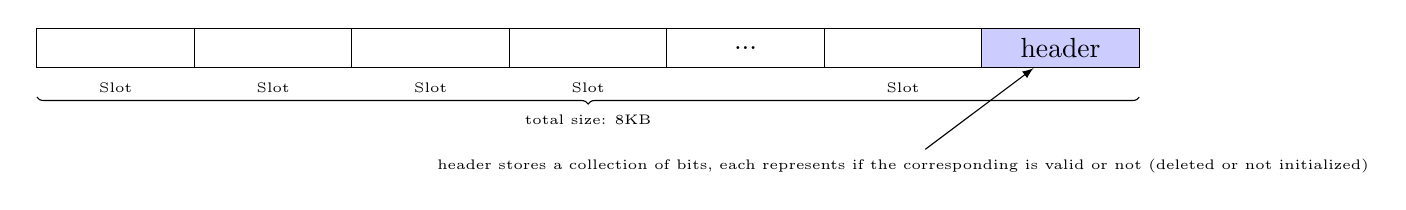
\begin{tikzpicture}[
            slot/.style={draw, minimum width=2cm, minimum height=0.5cm},
            brace/.style={decoration={brace, mirror},decorate}
        ]
        \foreach \x in {0, 2, ..., 6} {
            \node[slot] at (\x, 0) {};
            \node at (\x, -0.5) {\tiny{Slot}};
        }
        \node[slot] at (8, 0) {\text{...}};
        \node[slot] at (10, 0) {};
        \node at (10, -0.5) {\tiny{Slot}};
        \node[slot, fill=blue!20] (header) at (12, 0) {header};
        \node (headerd) at (10, -1.5) {\tiny{header stores a collection of bits, each represents if the corresponding is valid or not (deleted or not initialized)}};
        \path[->] (headerd) edge (header);
        % total size
        \node (start) at (-1, -0.5) {};
        \node (end) at (13, -0.5) {};
        \draw[brace] (start.south) -- node [below=3pt, pos=0.5] {\tiny{total size: 8KB}} (end.south);
        \end{tikzpicture}
        \end{center}

        % 2(b)
        \item 
        Suppose one page can fit $x$ tuples. We have
        $$ 34x + \frac{x}{8} \leq 8192 $$
        $$ x = \left\lfloor\frac{65536}{273}\right\rfloor = 240$$
        240 tuples fit on one page. We need $\left\lceil\frac{240}{8}\right\rceil = 30$ bytes for the page header. To fit 1000 tuples, we need $\left\lceil\frac{1000}{240}\right\rceil = 5$ pages

        % 2(c)
        \item schematic representation (3 variable length tuples stored):
        \begin{center}
        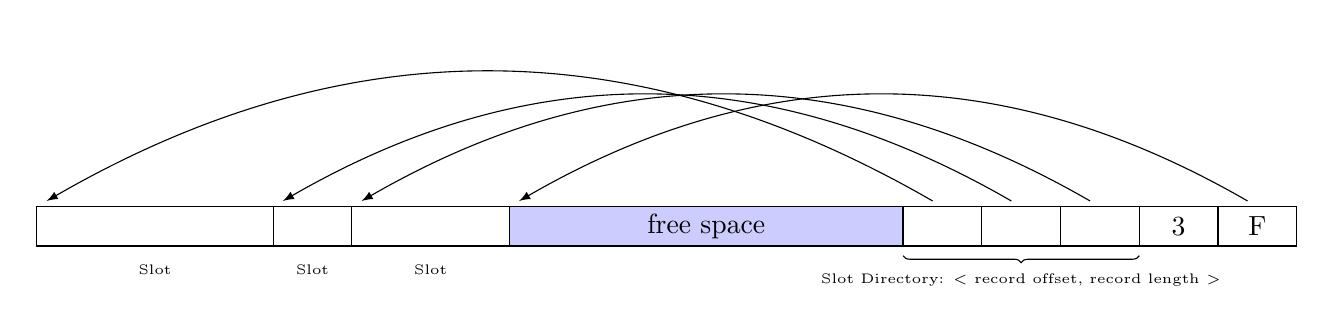
\begin{tikzpicture}[
            slot/.style={draw, minimum width=2cm, minimum height=0.5cm},
            brace/.style={decoration={brace, mirror},decorate}
        ]
            \node (onel) at (0, 0) {};
            \node (oner) at (3, -0.5) {};
            \node (twol) at (3, 0) {};
            \node (twor) at (4, -0.5) {};
            \node (threel) at (4, 0) {};
            \node (threer) at (6, -0.5) {};
            % label
            \node at (1.5, -0.8) {\tiny{Slot}};
            \node at (3.5, -0.8) {\tiny{Slot}};
            \node at (5, -0.8) {\tiny{Slot}};
            \node (freel) at (6, 0) {};
            \node (freer) at (11, -0.5) {};
            \node (sonel) at (11, 0) {};
            \node (soner) at (12, -0.5) {};
            \node (stwol) at (12, 0) {};
            \node (stwor) at (13, -0.5) {};
            \node (sthreel) at (13, 0) {};
            \node (sthreer) at (14, -0.5) {};
            \node (sthreel) at (13, 0) {};
            \node (sthreer) at (14, -0.5) {};
            \node (sthreel) at (13, 0) {};
            \node (sthreer) at (14, -0.5) {};
            \node (countl) at (14, 0) {};
            \node (countr) at (15, -0.5) {};
            \node (fl) at (15, 0) {};
            \node (fr) at (16, -0.5) {};
            \draw[draw=black] (onel) rectangle (oner);
            \draw[draw=black] (twol) rectangle (twor);
            \draw[draw=black] (threel) rectangle (threer);
            \draw[draw=black, fill=blue!20] (freel) rectangle (freer) node[midway] {free space};
            \draw[draw=black] (sonel) rectangle (soner);
            \draw[draw=black] (stwol) rectangle (stwor);
            \draw[draw=black] (sthreel) rectangle (sthreer);
            \draw[draw=black] (countl) rectangle (countr) node[midway] {3};
            \draw[draw=black] (fl) rectangle (fr) node[midway] {F};
            % paths
            \node (sone) at (11.5, 0) {};
            \node (stwo) at (12.5, 0) {};
            \node (sthree) at (13.5, 0) {};
            \node (sfree) at (15.5, 0) {};
            \path[->] (sone) edge [bend right] (onel);
            \path[->] (stwo) edge [bend right] (twol);
            \path[->] (sthree) edge [bend right] (threel);
            \path[->] (sfree) edge [bend right] (freel);
            \draw[brace] (freer.south) -- node [below=3pt, pos=0.5] {\tiny{Slot Directory: $<$ record offset, record length $>$}} (sthreer.south);
        \end{tikzpicture} 
        \end{center}
    \end{enumerate}
    
    %%% #3
    \item 
    \begin{enumerate}[listparindent=0.0em, itemsep=1em]
    \item 
    The project operator calls \texttt{next()}, which makes the sequential scan operator call \texttt{next()}. Then the heap file iterator interface gets called, which calls the \texttt{getPage()} and get the page data from the buffer pool manager.
    \item Since the buffer pool is initially empty, the first \texttt{next()} call will pull one whole page containing the data into the buffer pool. So the buffer pool will contain one cached page.
    \item The next \texttt{next()} call will get the data directly from the buffer pool's page. So the buffer pool still contains one page.
    \item We know from \# 2 one page contains 240 pages. So 1000 calls will need $\left\lceil\frac{1000}{240}\right\rceil = 5$ pages to be pulled into the buffer pool.
    \item Since the buffer pool can hold 10 pages. When the query completes, the buffer pool will contains 10 pages which hold the later $2400$ tuples.
    \end{enumerate} 
    \end{enumerate}
\end{document}
